\newpage
\pagestyle{empty} % Remueve los números de página

\vspace*{\fill}%Centra el contenido total en la hoja

\begin{center}

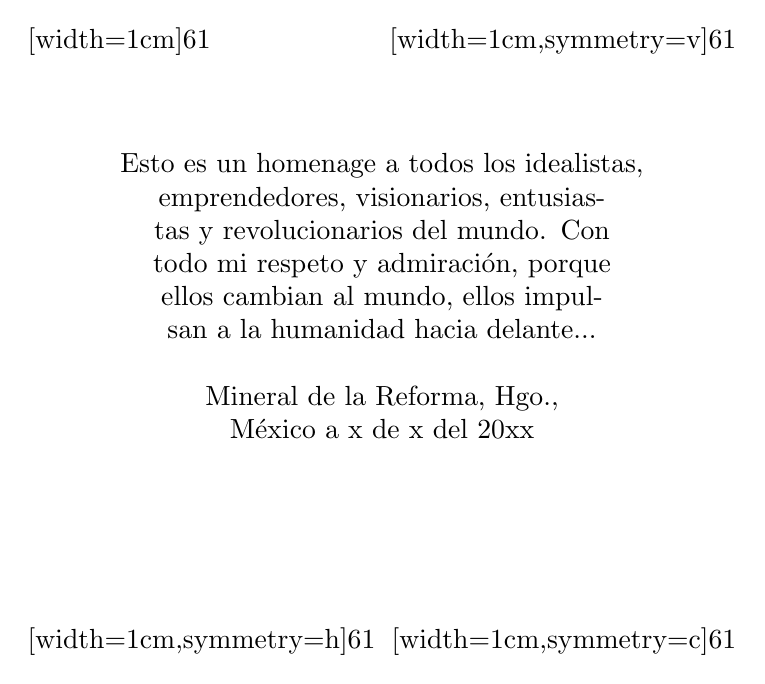
\begin{tikzpicture}[every node/.style={inner sep=0pt}]   
\node[text width=7cm,align=center](Text){%
\bigskip
% **************************************************
%\quotefont

Esto es un homenage a todos los idea\-lis\-tas, emprendedores, vi\-sio\-na\-rios, entusiastas y revolucionarios del mundo. Con todo mi respeto y admiración, porque ellos cambian al mundo, ellos impulsan a la humanidad hacia delante...\\
\bigskip
Mineral de la Reforma, Hgo., México a x de x del 20xx\\

\Huge
	\begin{center}
	\raisebox{-4pt}[10pt][10pt]{\textxswdown}
	\end{center}
% **************************************************
} ;
\node[shift={(-1cm,1cm)},anchor=north west](CNW)  at (Text.north west)
	             {\pgfornament[width=1cm]{61}};
\node[shift={(1cm,1cm)},anchor=north east](CNE)   at (Text.north east)
	             {\pgfornament[width=1cm,symmetry=v]{61}}; 
\node[shift={(-1cm,-1cm)},anchor=south west](CSW) at (Text.south west)
	             {\pgfornament[width=1cm,symmetry=h]{61}}; 
\node[shift={(1cm,-1cm)},anchor=south east](CSE)  at (Text.south east)   
	             {\pgfornament[width=1cm,symmetry=c]{61}};  
\pgfornamenthline{CNW}{CNE}{north}{88}
\pgfornamenthline{CSW}{CSE}{south}{88}
\pgfornamentvline{CNW}{CSW}{west}{88}
\pgfornamentvline{CNE}{CSE}{east}{88} 
\end{tikzpicture}

\end{center}

\vspace*{\fill}%Centra el contenido total en la hoja


